\documentclass[varwidth]{standalone}

\usepackage{amsmath}
\usepackage[dvipsnames]{xcolor}
\usepackage{tikz}
\usetikzlibrary{arrows.meta}
\usetikzlibrary{backgrounds}
\usetikzlibrary{calc}
\usetikzlibrary{fit}
\usetikzlibrary{positioning}
\usetikzlibrary{patterns}
\usetikzlibrary{shapes}
\usetikzlibrary{shapes.misc}


\begin{document}

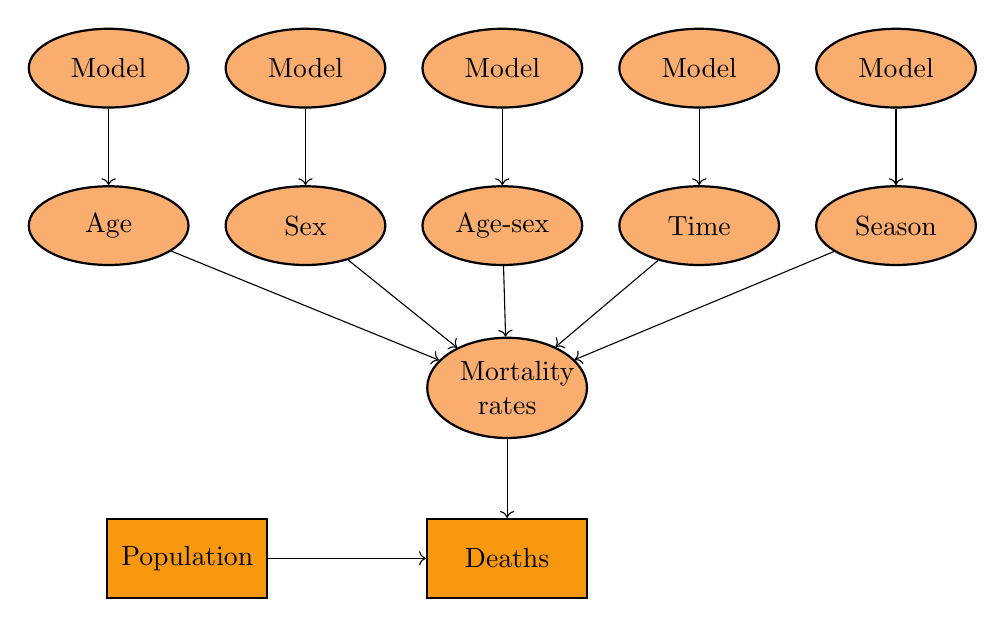
\begin{tikzpicture}
  [
    node distance = 1.5cm and 2cm,
    node/.style = {thick, draw, text width = 1.2cm,
                  minimum height = 1cm, align = center},
    obs/.style = {node, rectangle, text width = 1.8cm, fill=YellowOrange},
    unobs/.style = {node, ellipse, fill=Apricot},
    arrow/.style  = {> = stealth, thick, length=8pt},
  ]
    
  \node[obs] (y) {Deaths};
  \node[obs] [left = of y] (w) {Population}
  edge[->](y);

  \node[unobs][above = of y, yshift = -0.5cm] (mu) {Mortality rates}
    edge[->](y);

    \node[unobs] [above left of = mu, xshift = -4cm, yshift = 1cm] (beta_age) {Age}
      edge[->](mu);
    \node[unobs] [right of = beta_age, xshift = 1cm] (beta_sex) {Sex}
      edge[->](mu);
    \node[unobs] [right of = beta_sex, xshift = 1cm] (beta_agesex) {Age-sex}
      edge[->](mu);
    \node[unobs] [right of = beta_agesex, xshift = 1cm] (beta_time) {Time}
      edge[->](mu);
    \node[unobs] [right of = beta_time, xshift = 1cm] (beta_season) {Season}
      edge[->](mu);

    \node[unobs] [above of = beta_age, yshift = 0.5cm] (pi_age) {Model}
      edge[->](beta_age);
    \node[unobs] [above of = beta_sex, yshift = 0.5cm] (pi_sex) {Model}
      edge[->](beta_sex);
    \node[unobs] [above of = beta_agesex, yshift = 0.5cm] (pi_agesex) {Model}
      edge[->](beta_agesex);
    \node[unobs] [above of = beta_time, yshift = 0.5cm] (pi_time) {Model}
      edge[->](beta_time);
    \node[unobs] [above of = beta_season, yshift = 0.5cm] (pi_season) {Model}
      edge[->](beta_season);
    
  \end{tikzpicture}

  \end{document}